\documentclass{beamer}

\usepackage{beamerthemesplit}
\usepackage{verbatim}

\usetheme{default}
%\usetheme{Pittsburgh}
%\usecolortheme{seagull}
%\usecolortheme{seahorse}
%\usecolortheme{beaver}
\usecolortheme{mule}

\usefonttheme{serif}

%\DeclareGraphicsExtensions{.pdf,.png,.jpg}

\newcommand{\snT}{$(S/N)_{\textrm{size}}$}
%\newcommand{\snT}{$\left( \frac{S}{N}\right)_{\textrm{size}}$}
\newcommand{\snflux}{$(S/N)_{\textrm{flux}}$}
%\newcommand{\snflux}{$\left( \frac{S}{N}\right)_{\textrm{flux}}$}

\newcommand{\lensfit}{\texttt{LENSFIT}}
\newcommand{\numba}{\texttt{Numba}}
\newcommand{\python}{\texttt{Python}}
\newcommand{\ngmix}{\texttt{ngmix}}
\newcommand{\shear}{{\bf g}}
\newcommand{\redmapper}{redMaPPer}

\newcommand{\prelim}{{\bf{\it Preliminary}}}

\definecolor{gold}{rgb}{1.,0.84,0.}


\title{Measuring Dark Matter and Dark Energy with Gravitational Lensing}
\author{Erin Sheldon}
\institute{Brookhaven National Laboratory}

% http://texblog.net/latex-archive/plaintex/beamer-footline-frame-number/
% to add the page (frame ) number and not screw up the bottom line
% works for split themes?
\expandafter\def\expandafter\insertshorttitle\expandafter{%
      \insertshorttitle\hfill%
        \insertframenumber\,/\,\inserttotalframenumber}

% suppress navigation bar
\beamertemplatenavigationsymbolsempty
\setbeamertemplate{footline}{}

\begin{document}

\frame{\titlepage}


\frame
{
    \frametitle{Outline}

    \begin{itemize}

        \item Gravitational Lensing

        \item Dark Matter

            \begin{itemize}
                \item What was known before lensing
                \item My measurements using lensing
            \end{itemize}

        \item Dark Energy
            \begin{itemize}
                \item The little bit we know
                \item Lensing and Dark Energy
                \item Dark Energy Survey, \prelim\ results
            \end{itemize}

        \item LSST

    \end{itemize}


}

\frame
{

    {\em Do not Bodies act upon light at a distance, and by their action bend its Rays;
    and is not this action } (caeteris paribus) {\em strongest at the least distance?}
    \newline

    \hfill - Isaac Newton (Query I, Opticks, 1704)
}

\frame
{
    \frametitle{Gravitational Lensing}

    \begin{itemize}

        \item Newton's first Query, Opticks, 1704
            \begin{itemize}
                \item One can incorrectly ``cancel'' the zero masses and predict
                    some light deflection
            \end{itemize}

        \item Einstein 1911
            \begin{itemize}

                \item Equivalence principle

                \item Observers in free fall experience an inertial frame.  The
                    light appears to follow straight lines: the light falls
                    with them.

            \end{itemize}

        \item Einstein 1915
            \begin{itemize}
                \item Full result from general relativity, factor of two larger
            \end{itemize}


    \end{itemize}

}


%{
%	\definecolor{mblack}{RGB}{0,0,0}
%    \setbeamertemplate{background canvas}[vertical shading][bottom=black,top=black]
	
    \frame
    {
        \frametitle{1919 Eclipse}

        %\fontsize{9}{0.8\baselineskip}
        \begin{columns}
            \begin{column}{0.5\textwidth}    
                \begin{itemize}

                    \item Einstein predicted the small deflection of light from
                        stars whose light passes very near the sun.

                    \item Eddington and colleagues observed the predicted
                        deflection in the 1919 eclipse.

                \end{itemize}
            \end{column}
            \begin{column}{0.5\textwidth}
                \begin{center}
                    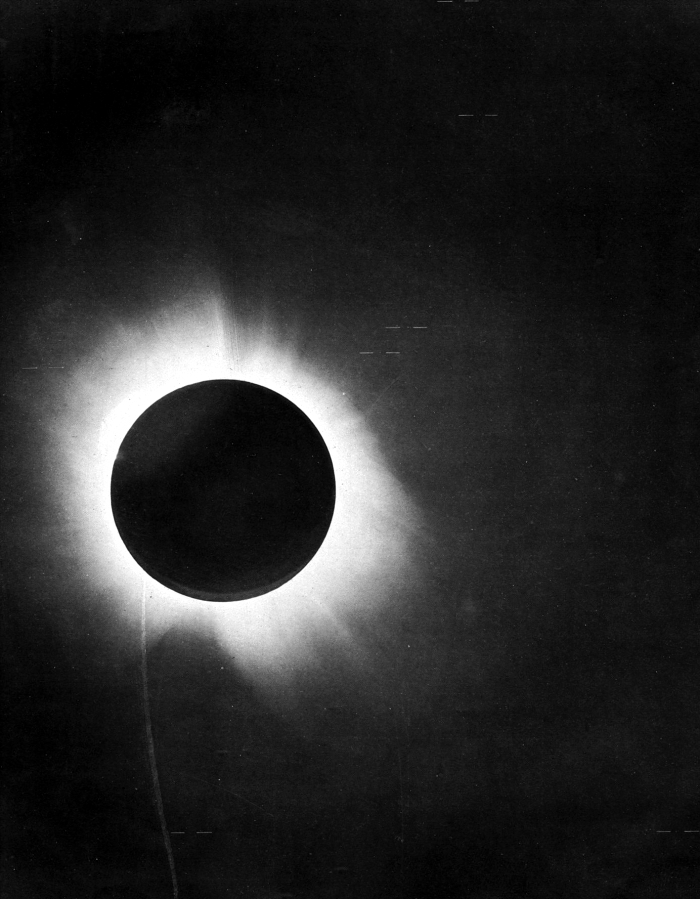
\includegraphics[width=\textwidth]{1919_eclipse_positive.jpg}
                    \newline
                    {\tiny Dyson, Eddington, Davidson 1919}
                \end{center}
            \end{column}
        \end{columns}
    }

%	\definecolor{mblack}{RGB}{50,50,50}
%    \setbeamertemplate{background canvas}[vertical shading][bottom=mgray,top=mblack]

%}

\frame
{
    \frametitle{Lensing Geometry}

    \begin{center}
        
\includegraphics[scale=0.4]{lens_geometry_invert.pdf}
        \newline
        For a point mass, the deflection depends on impact
        prameter as
        \newline
        {\huge {\color{gold} $\alpha \propto \frac{M}{b}$ }}
    \end{center}
}



\frame
{
    \frametitle{Twin Quasar 0957+0561}

    %\fontsize{9}{0.8\baselineskip}
    \begin{columns}
        \begin{column}{0.5\textwidth}    
            \begin{itemize}

                \item Two quasars discovered in 1979 (Walsh, Carswell, Weyman)

                \item Extremely close together, nearly identical spectrum and redshift

                \item Time variations in image A appear in image B also, but 14 months later.

                \item Two images of the same object!
                    
            \end{itemize}
        \end{column}
        \begin{column}{0.5\textwidth}
            \begin{center}
                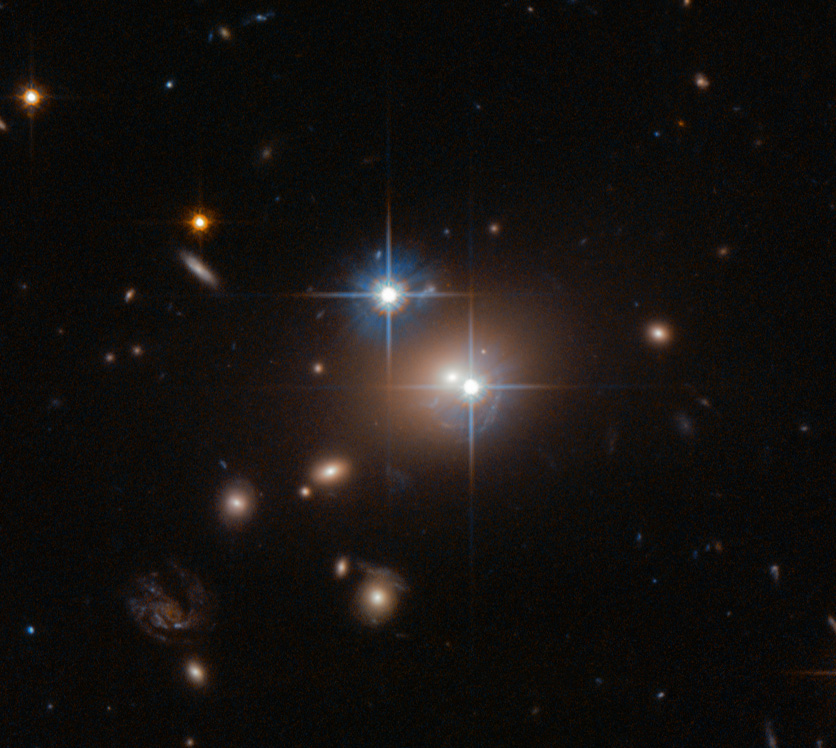
\includegraphics[width=\textwidth]{QSO_B0957+0561-crop.jpg}
                \newline
                {\tiny ESA/Hubble \& NASA}
            \end{center}
        \end{column}
    \end{columns}
}

\frame
{
    \frametitle{Lensing Geometry}

    \begin{center}
        
\includegraphics[scale=0.5]{lens_geometry_invert.pdf}
    \end{center}
}


{
	\definecolor{mblack}{RGB}{0,0,0}
    \setbeamertemplate{background canvas}[vertical shading][bottom=black,top=black]
	
    \frame
    {
        \frametitle{Einstein Ring: The ``Horseshoe''}

        \begin{center}
            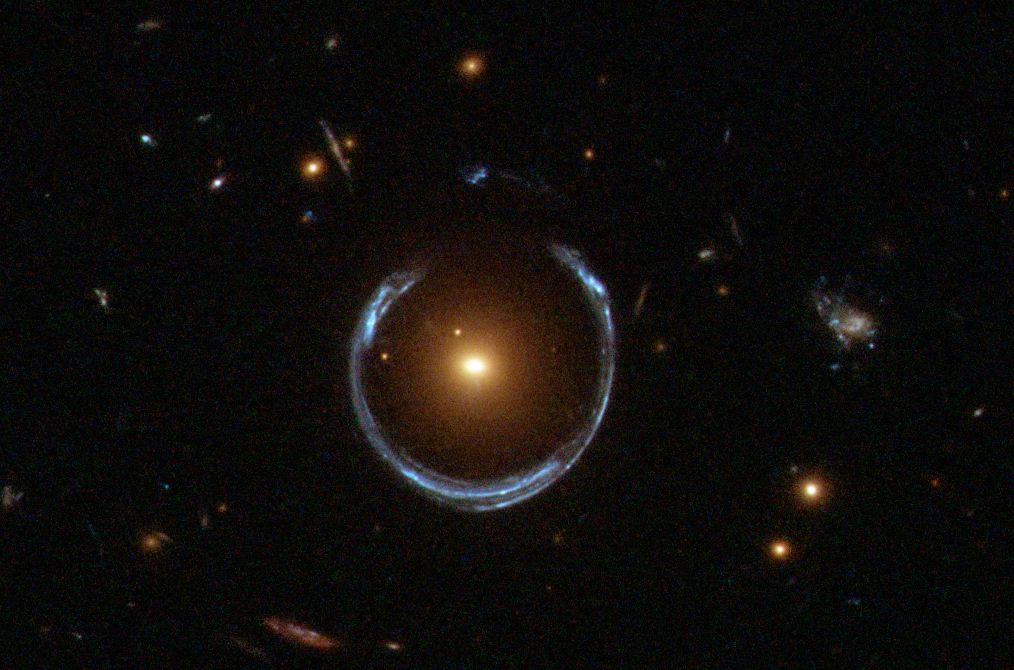
\includegraphics[height=0.7\textheight]{A_Horseshoe_Einstein_Ring_from_Hubble.JPG}

            {\tiny \hfill ESA/Hubble \& NASA}
        \end{center}
    }

	\definecolor{mblack}{RGB}{50,50,50}
    \setbeamertemplate{background canvas}[vertical shading][bottom=mgray,top=mblack]

}

{
	\definecolor{mblack}{RGB}{0,0,0}
    \setbeamertemplate{background canvas}[vertical shading][bottom=black,top=black]
	
    \frame
    {
        \frametitle{Lensing by Galaxy Clusters: Abell 1689}

        \begin{center}
            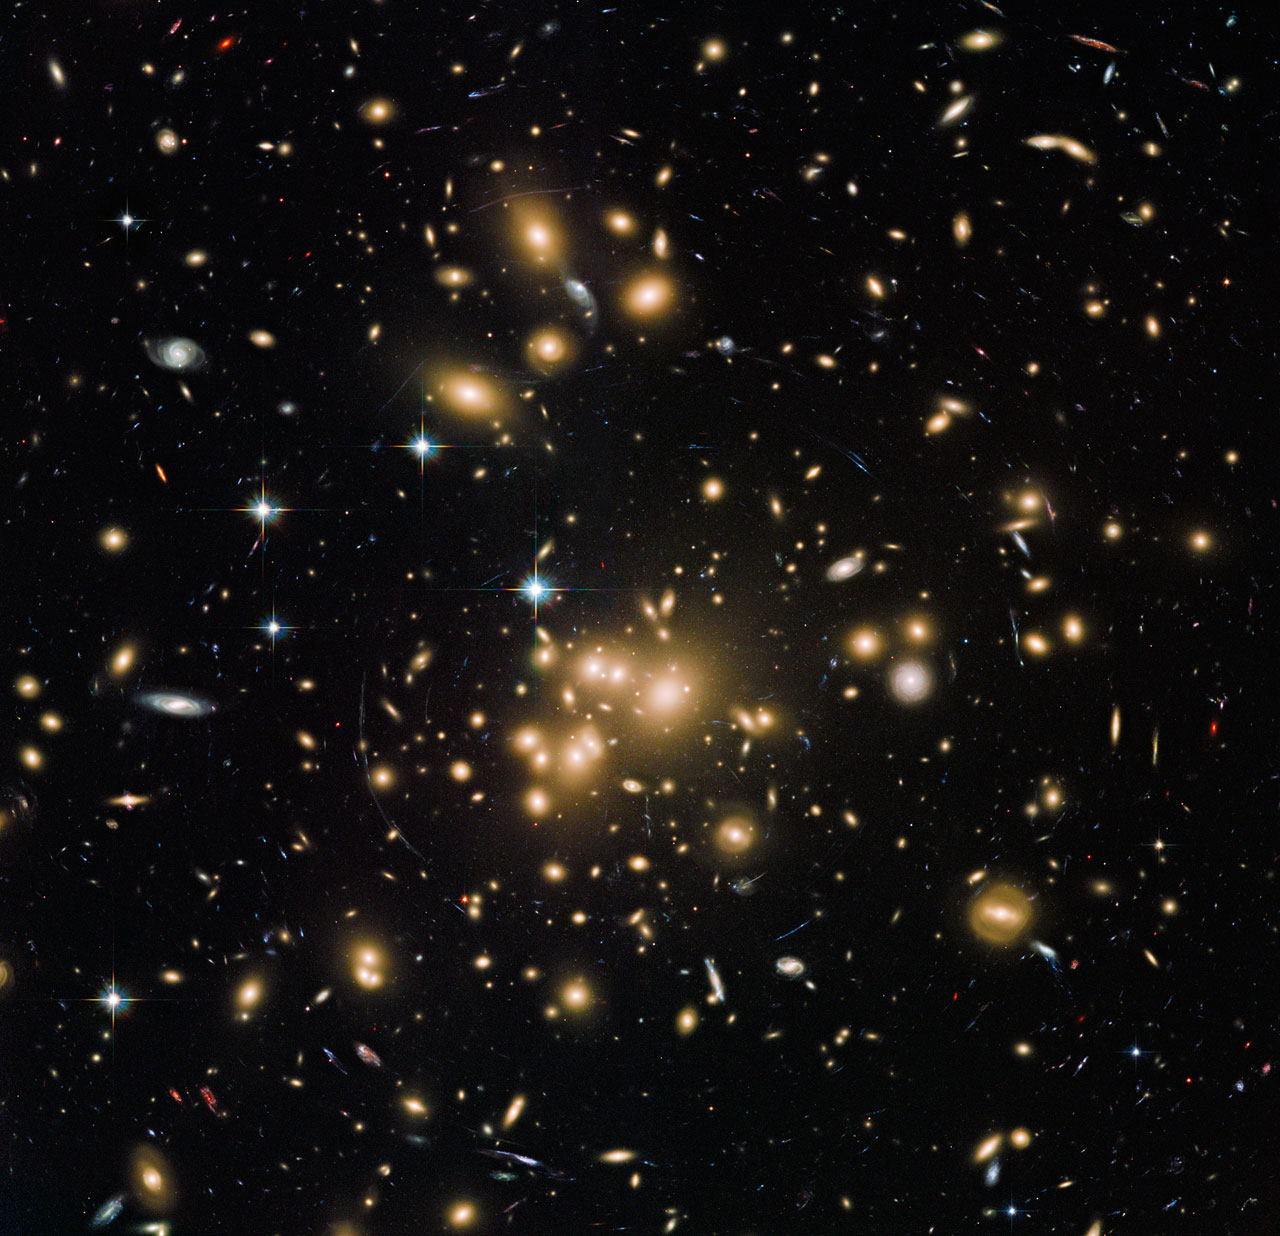
\includegraphics[height=0.8\textheight]{abell1689_hubble_1280.jpg}

            {\tiny \hfill NASA, ESA, STScI/AURA, J. Blakeslee, H. Ford}
        \end{center}
    }

	\definecolor{mblack}{RGB}{50,50,50}
    \setbeamertemplate{background canvas}[vertical shading][bottom=mgray,top=mblack]

}

{
	\definecolor{mblack}{RGB}{0,0,0}
    \setbeamertemplate{background canvas}[vertical shading][bottom=black,top=black]
	
    \frame
    {
        \begin{center}
            \includegraphics[height=0.9\textheight]{abell1689-details.pdf}
        \end{center}
    }

	\definecolor{mblack}{RGB}{50,50,50}
    \setbeamertemplate{background canvas}[vertical shading][bottom=mgray,top=mblack]

}

{
	\definecolor{mblack}{RGB}{0,0,0}
    \setbeamertemplate{background canvas}[vertical shading][bottom=black,top=black]
	
    \frame
    {
        \frametitle{Shear Illustration}
        \begin{center}
            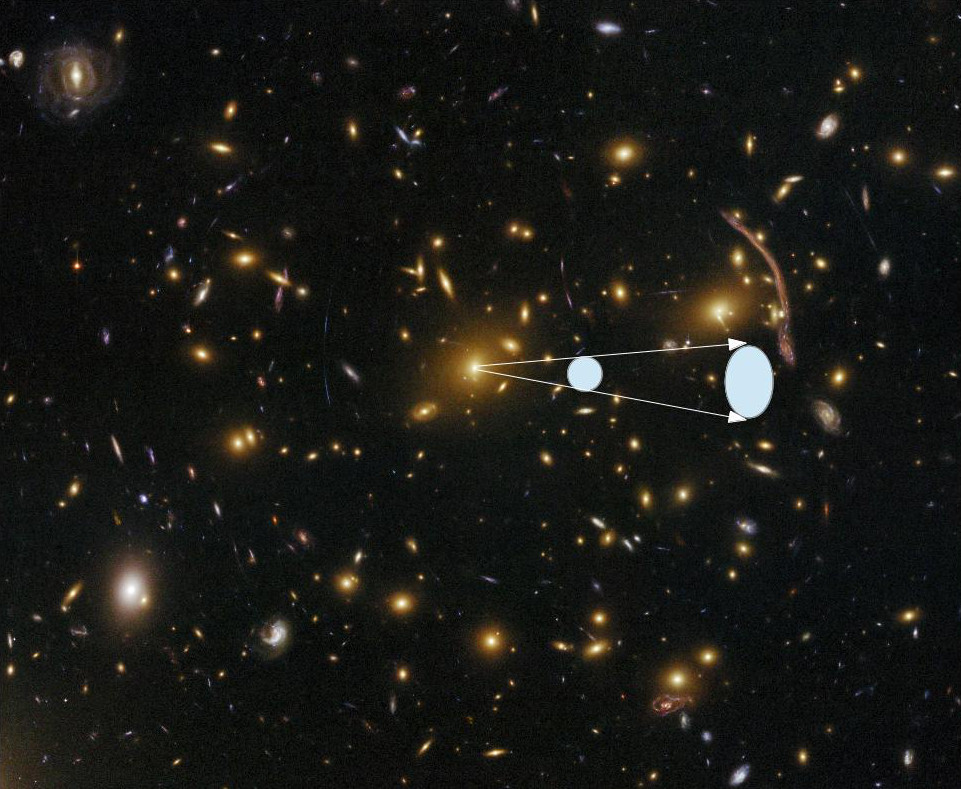
\includegraphics[height=0.8\textheight]{shear-illustration-nowhite.jpg}
        \end{center}
    }

	\definecolor{mblack}{RGB}{50,50,50}
    \setbeamertemplate{background canvas}[vertical shading][bottom=mgray,top=mblack]

}

	
\frame
{
    \frametitle{Shear Illustration}

    \begin{columns}
        \begin{column}{0.5\textwidth}    
            \begin{itemize}

                \item The shape of extended background sources is changed.

                \item The differential deflections across the surface
                    of the background image produces a shear.

                \item For strong lensing a round source becomes a ``banana''

                \item For {\color{gold} weak lensing} a round source becomes slightly elliptical

            \end{itemize}
        \end{column}
        \begin{column}{0.5\textwidth}
            \begin{center}
                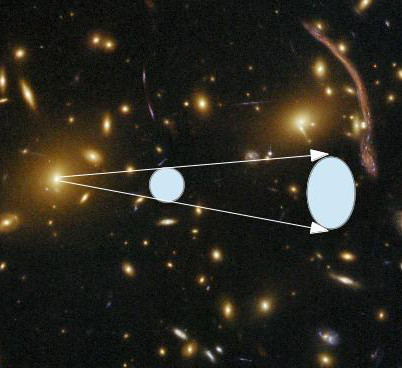
\includegraphics[width=\textwidth]{shear-illustration-crop2.jpg}
                \newline
                {\small Tangential Shear}
            \end{center}
        \end{column}
    \end{columns}
}

\frame
{
    \frametitle{Weak Lensing}

    \begin{columns}
        \begin{column}{0.5\textwidth}    
            \begin{itemize}

                \item Strong lensing requires special, fortuitous alignments.
                    Not that useful as a general tool

                \item But everything is lensed slightly, and the {\color{gold} tangential shear}
                    pattern is imprinted all over the sky.

                \item Taking a statistical approach, we can study the mass
                    distribution around any set of objects.

            \end{itemize}
        \end{column}
        \begin{column}{0.5\textwidth}
            \begin{center}
                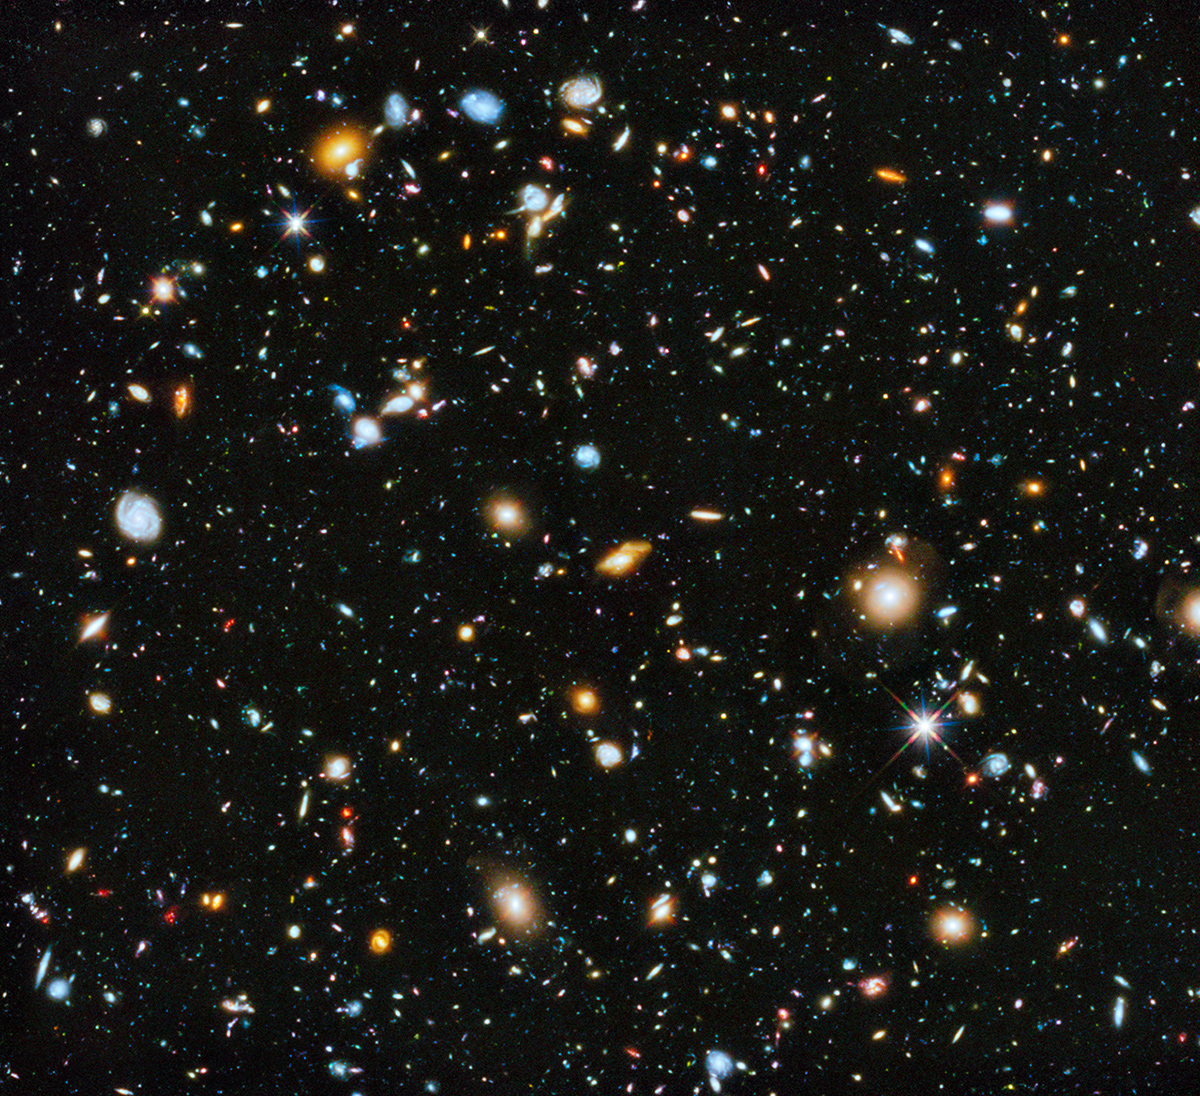
\includegraphics[width=\textwidth]{hubble-ultra-deep.jpg}
                \newline
                {\tiny  NASA/ESA, Teplitz et al.}
            \end{center}
        \end{column}
    \end{columns}
}

\frame
{
    \frametitle{Dark Matter}

    \begin{columns}
        \begin{column}{0.5\textwidth}    
            \begin{itemize}

                \item Fritz Zwicky 1937

                \item The galaxies in the Coma cluster moving far too fast.

                \item Implied binding mass $\sim$ 100 times the mass in stars

            \end{itemize}
        \end{column}
        \begin{column}{0.5\textwidth}
            \begin{center}
                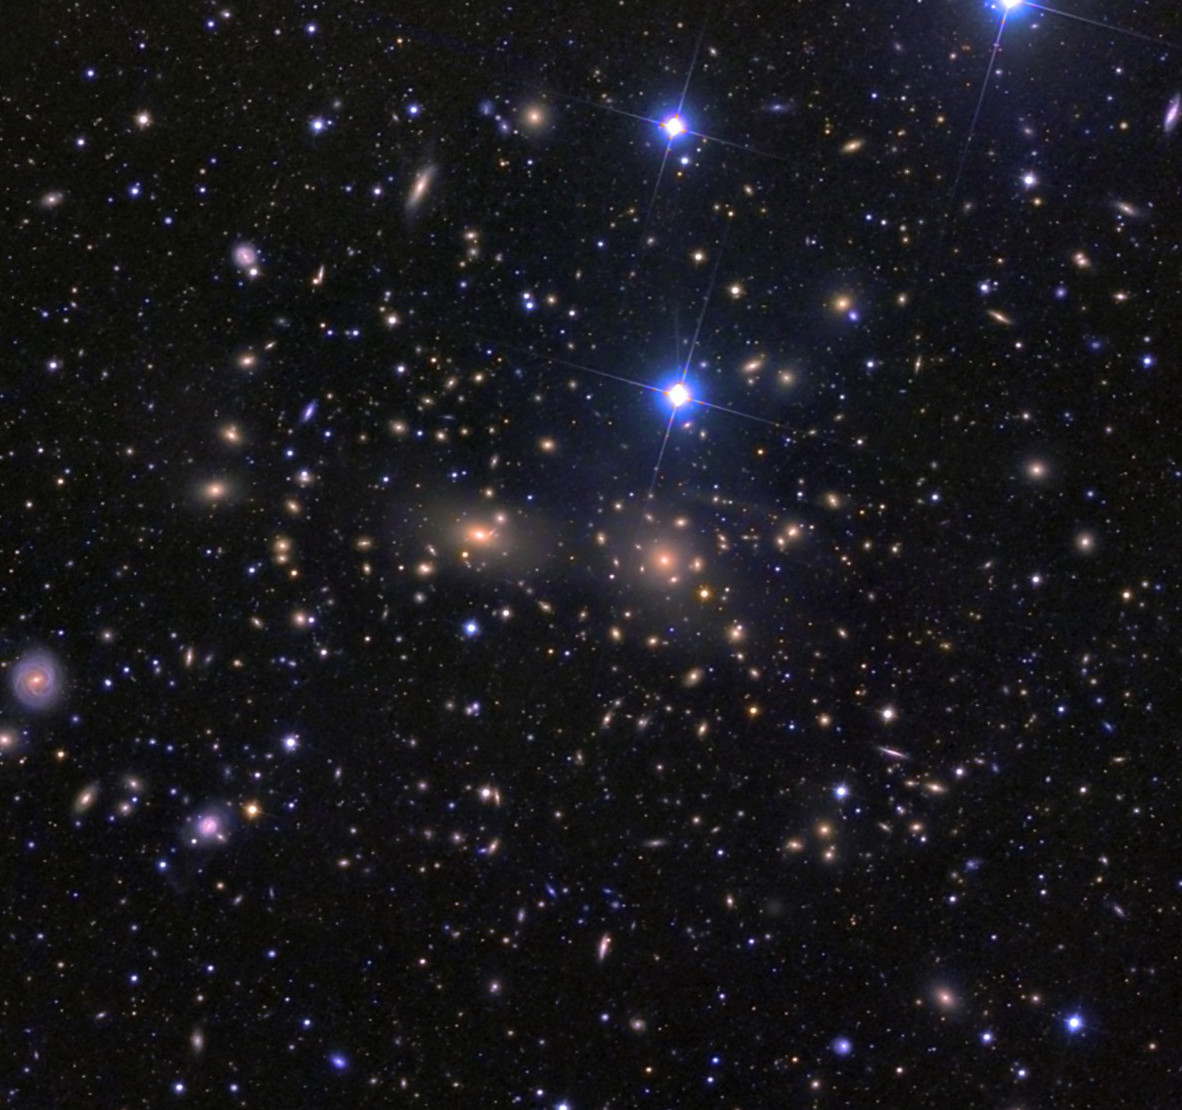
\includegraphics[width=\textwidth]{comacluster_rowe_big_crop.jpg}
                \newline
                {\tiny Dean Rowe}
            \end{center}
        \end{column}
    \end{columns}
}

\frame
{

    {\em The observation of such gravitational lens effects promises to furnish us with
    the simplest and most accurate determination of nebular masses.}
    \newline

    \hfill - Fritz Zwicky, 1937
}


\frame
{
    \frametitle{Dark Matter: Galaxy Rotation Curves}

    \begin{columns}
        \begin{column}{0.5\textwidth}    
            \begin{itemize}

                \item Rubin studied the rotation curves of galaxies in the 70s

                \item The light of galaxies falls exponentially with radius.

                \item The mass implied by the velocities falls like a power law

                \item Extrapolation seemed to imply the mass continued well
                    beyond the region of visible stars

            \end{itemize}
        \end{column}
        \begin{column}{0.5\textwidth}
            \begin{center}
                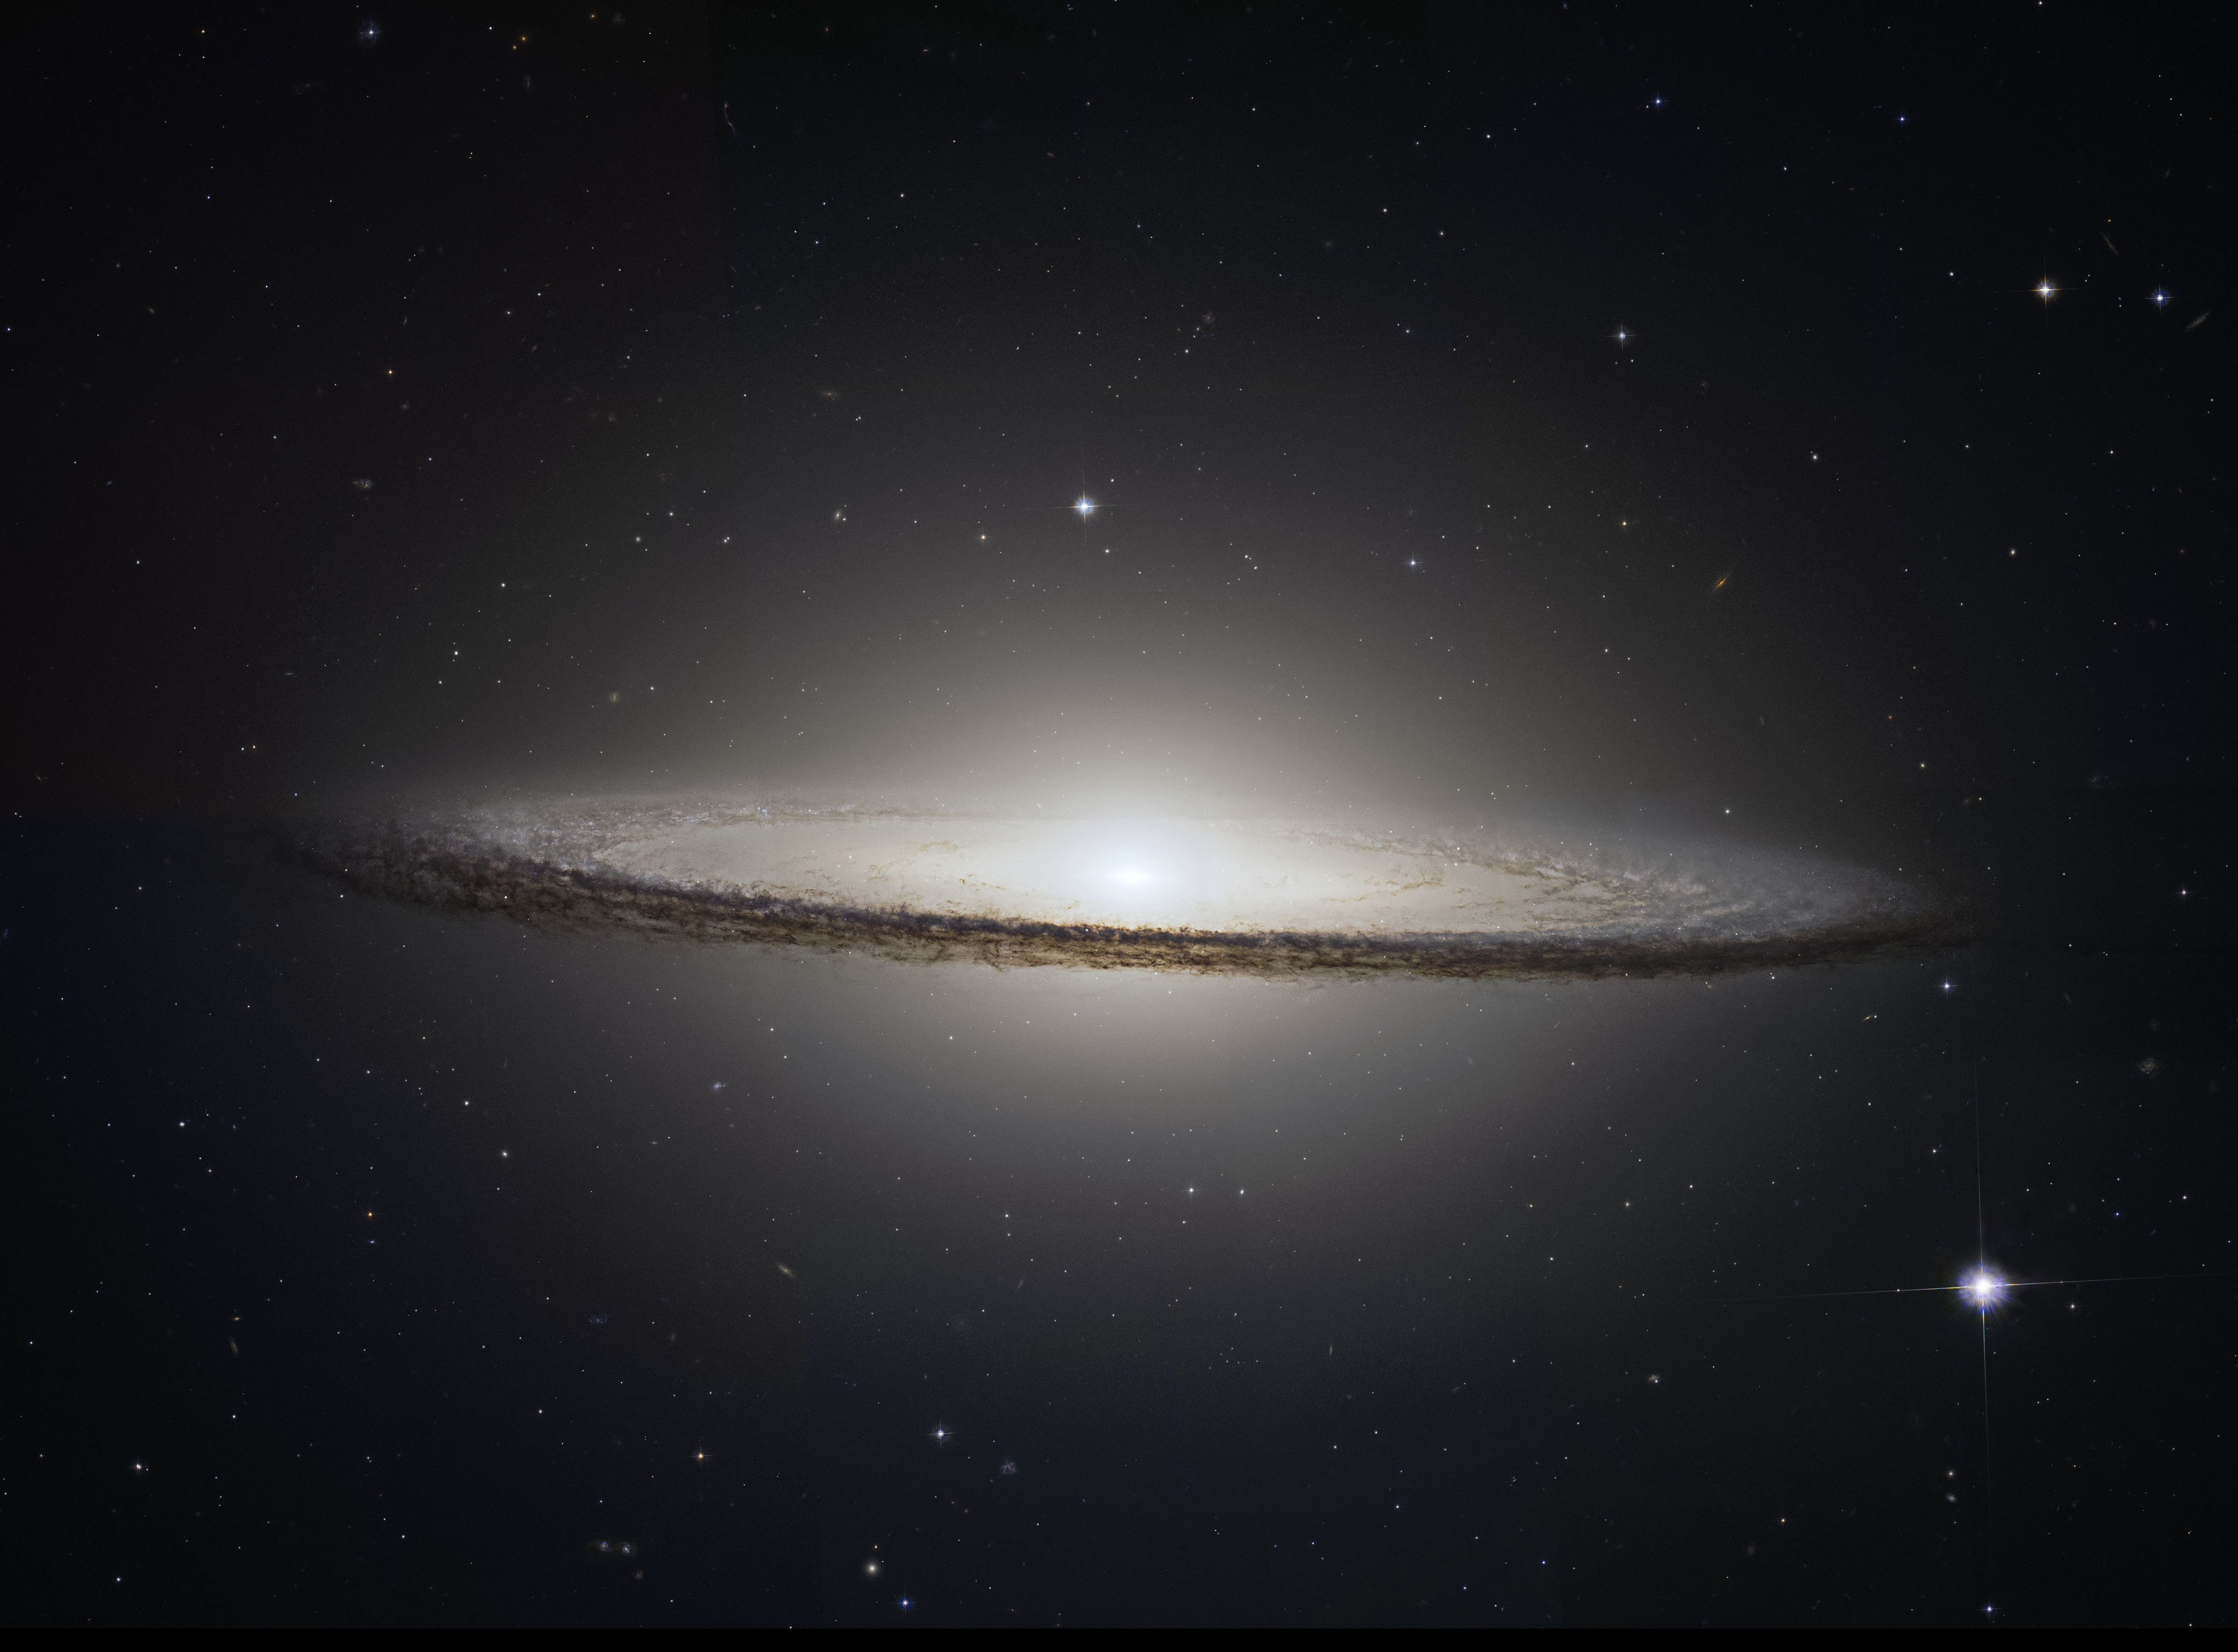
\includegraphics[width=0.8\textwidth]{m104-2013-03-01-HLA-5238-HLA-crop.jpg}
                \newline
                {\tiny NASA/ESA}

                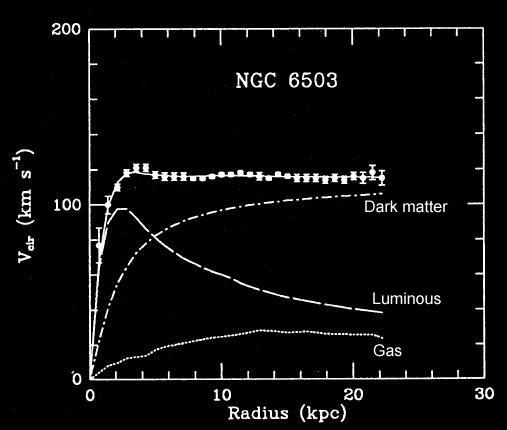
\includegraphics[width=0.8\textwidth]{ngc-6503-rotation-curve.jpg}
                \newline
                {\tiny Begeman, Broels and Sanders (1991)}
            \end{center}
        \end{column}
    \end{columns}
}

\frame
{
    \frametitle{Cold Dark Matter (CDM)}

    \begin{itemize}

        \item Some form of matter that does not significantly emit or absorb light

        \item Favored idea is an elementary particle, weakly interacting

        \item So far CDM explains everything we see, as I will discuss below

    \end{itemize}


}

\frame
{
    \frametitle{Early Successes of CDM}

    \begin{itemize}

        \item Explains rotation curves of galaxies

        \item Explains the dynamics of galaxy clusters

        \item Explains the large scale distribution of galaxies: without it we
          would predict a wildly different universe

        \item Essential component needed to explain the cosmic microwave
          background

    \end{itemize}

}

\frame
{
    \frametitle{Predictions of CDM}

    \begin{itemize}

        \item  ``Universal'' radial profile of gravitationally bound dark matter
            structures, ``halos'' (NFW)
            \begin{itemize}
                \item Running power law with one free parameter for shape
                \item Mass extends orders of magnitude farther beyond visible portion of galaxy,
                    merges with neighbors
            \end{itemize}



          %\item  show picture
          %\item  say from first principles can prediction ~power law nature, but
          %  details are interesting (broken power law)

        \item  Dark matter should be distributed smoothly throughout the
            universe, unlike dissipative baryons clumped in galaxies.

            %\item  correlations in this field known from first principles on the
            %  largest scales

    \end{itemize}

}

\frame
{
    \frametitle{Predictions of CDM}

    \fontsize{9}{0.8\baselineskip}
    \begin{columns}
        \begin{column}{0.5\textwidth}    
            \begin{itemize}

                \item  ``Universal'' radial profile of gravitationally bound dark matter
                    structures, ``halos'' {\color{gold} (NFW)}

                    %\begin{itemize}
                        \item Running power law with one free parameter for shape

                        \item Mass extends orders of magnitude farther than visible portion of galaxy,
                            merges with neighbors
                    %\end{itemize}

                \item  Dark matter distributed smoothly throughout the
                    universe, unlike dissipative baryons clumped in galaxies.

                {\tiny 1pc = 3.2 ly}

            \end{itemize}
        \end{column}
        \begin{column}{0.5\textwidth}
            \begin{center}
                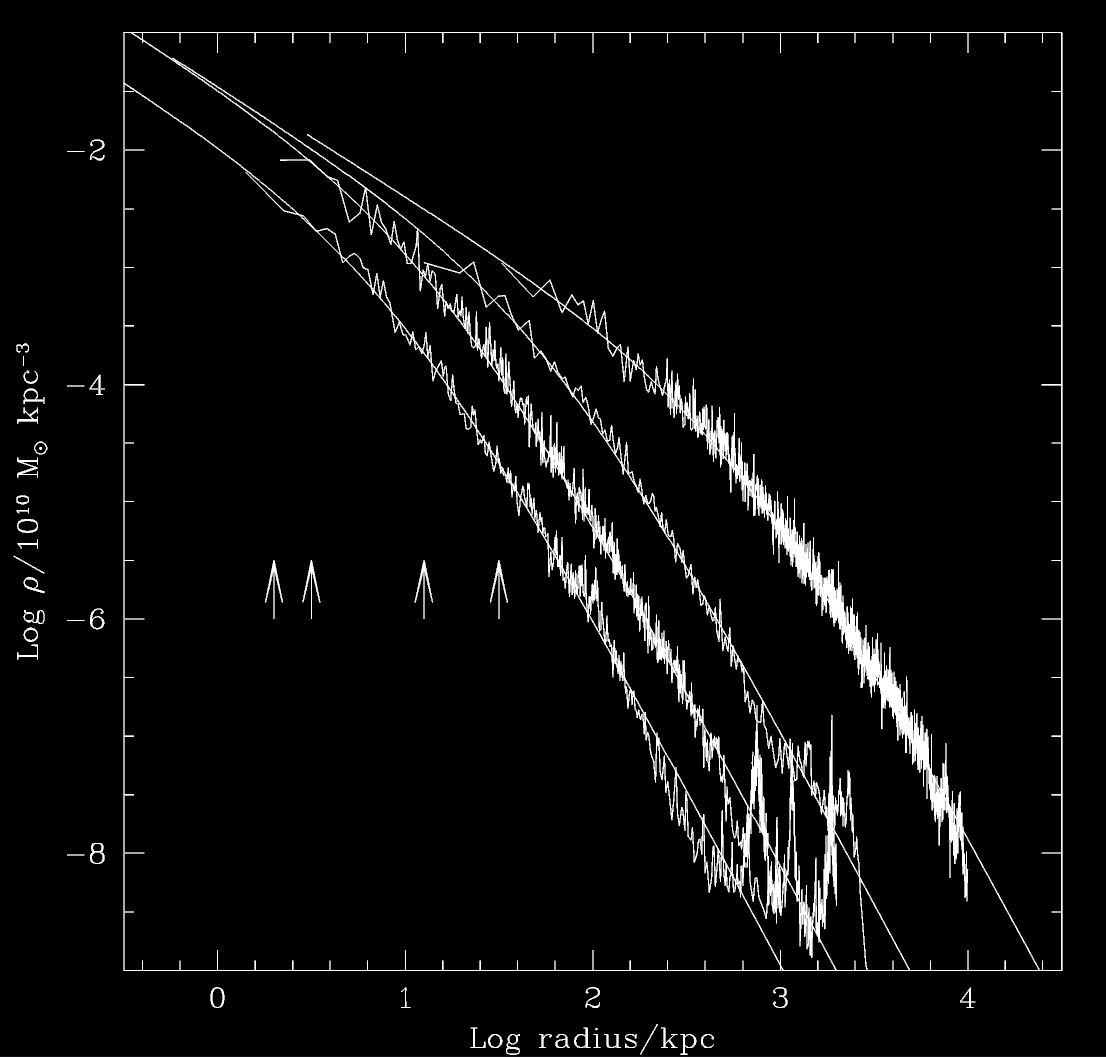
\includegraphics[width=\textwidth]{nfw.png}
                \newline
                {\tiny Navarro, Frenk, White 1996}
            \end{center}
        \end{column}
    \end{columns}
}


\frame
{
    \frametitle{Limits of dynamical approaches}

    \begin{columns}
        \begin{column}{0.5\textwidth}    
            \begin{itemize}

                \item visible tracers are required
                \item cannot trace out the orbits, the timescales are too long
                \item assumptions must be made about the dynamical state of the system
                \item limits the scale over which it this can be used

            \end{itemize}
        \end{column}
        \begin{column}{0.5\textwidth}
            \begin{center}
                {\small Scale 10 kpc}
                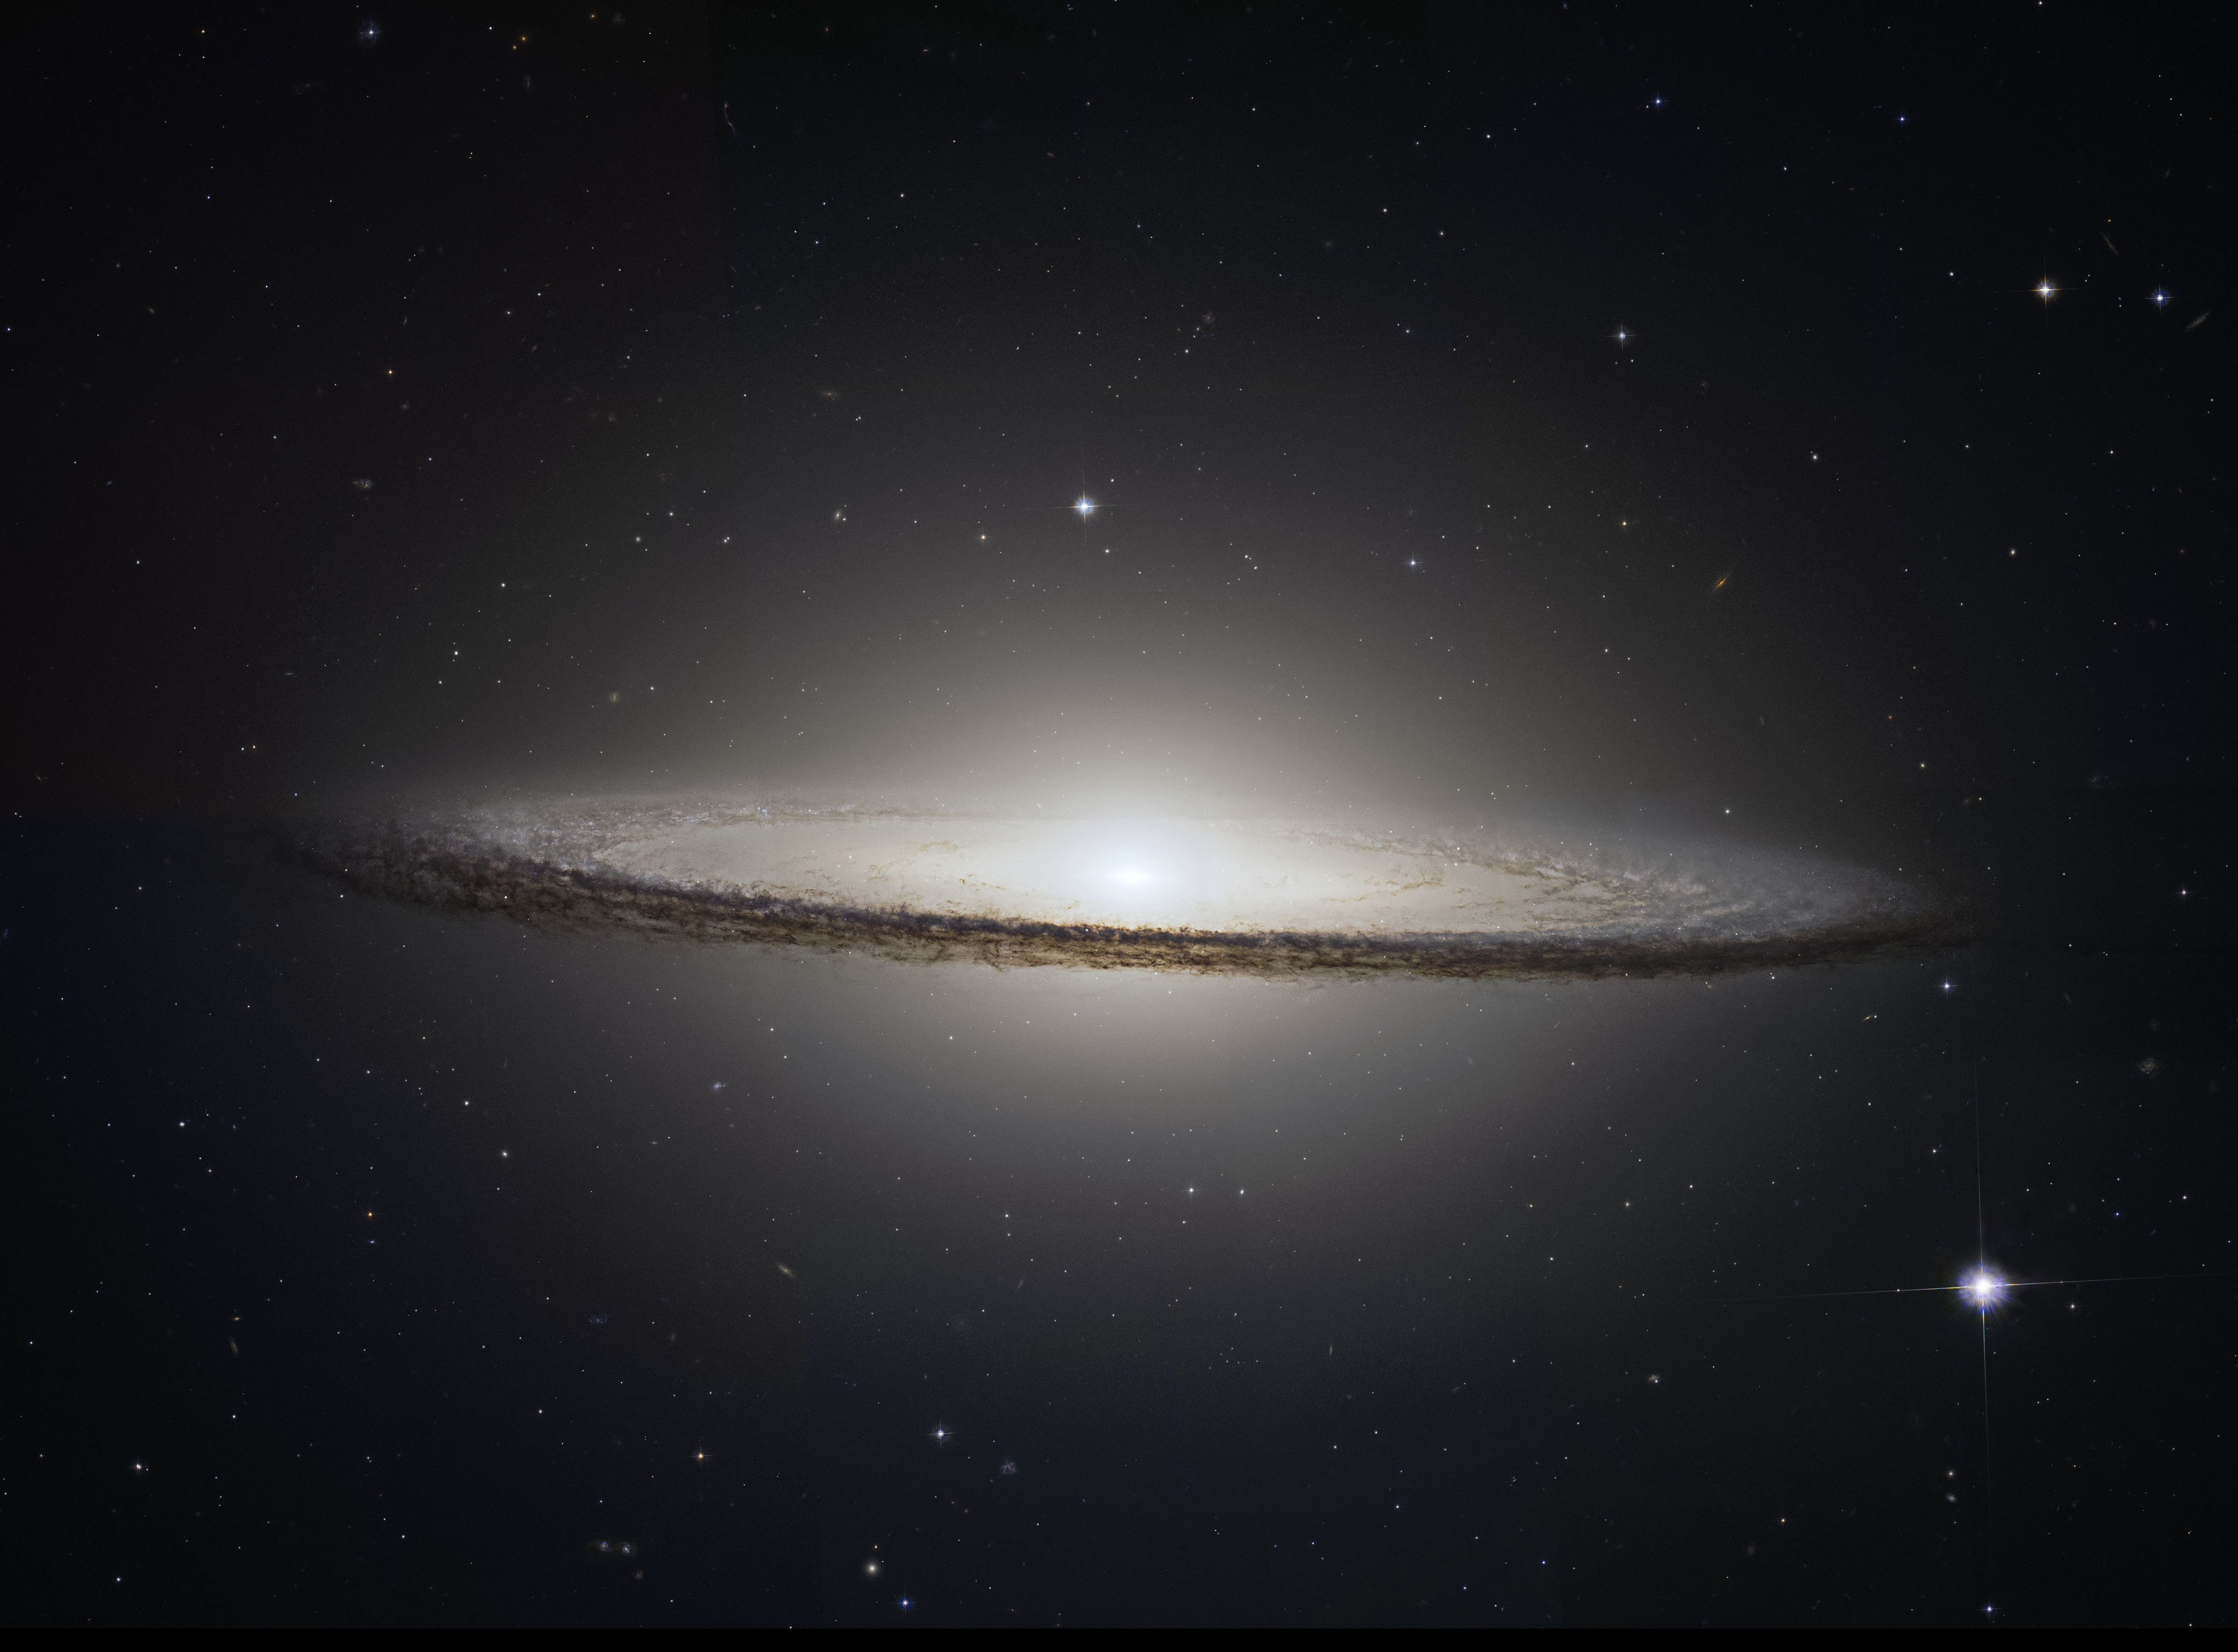
\includegraphics[width=\textwidth]{m104-2013-03-01-HLA-5238-HLA-crop.jpg}
                \newline
                {\tiny NASA/ESA}
            \end{center}
        \end{column}
    \end{columns}
}

\frame
{
    \frametitle{Weak Lensing is a Better Option}

    \begin{columns}
        \begin{column}{0.5\textwidth}    
            \begin{itemize}

                \item The weak effect can be observed anywhere
                \item The distribution of matter can be studied on a large range of scales
                \begin{itemize}
                    \item galaxies, galaxy clusters, bound objects
                    \item structure on the largest scales in the universe
                \end{itemize}

            \end{itemize}
        \end{column}
        \begin{column}{0.5\textwidth}
            \begin{center}
                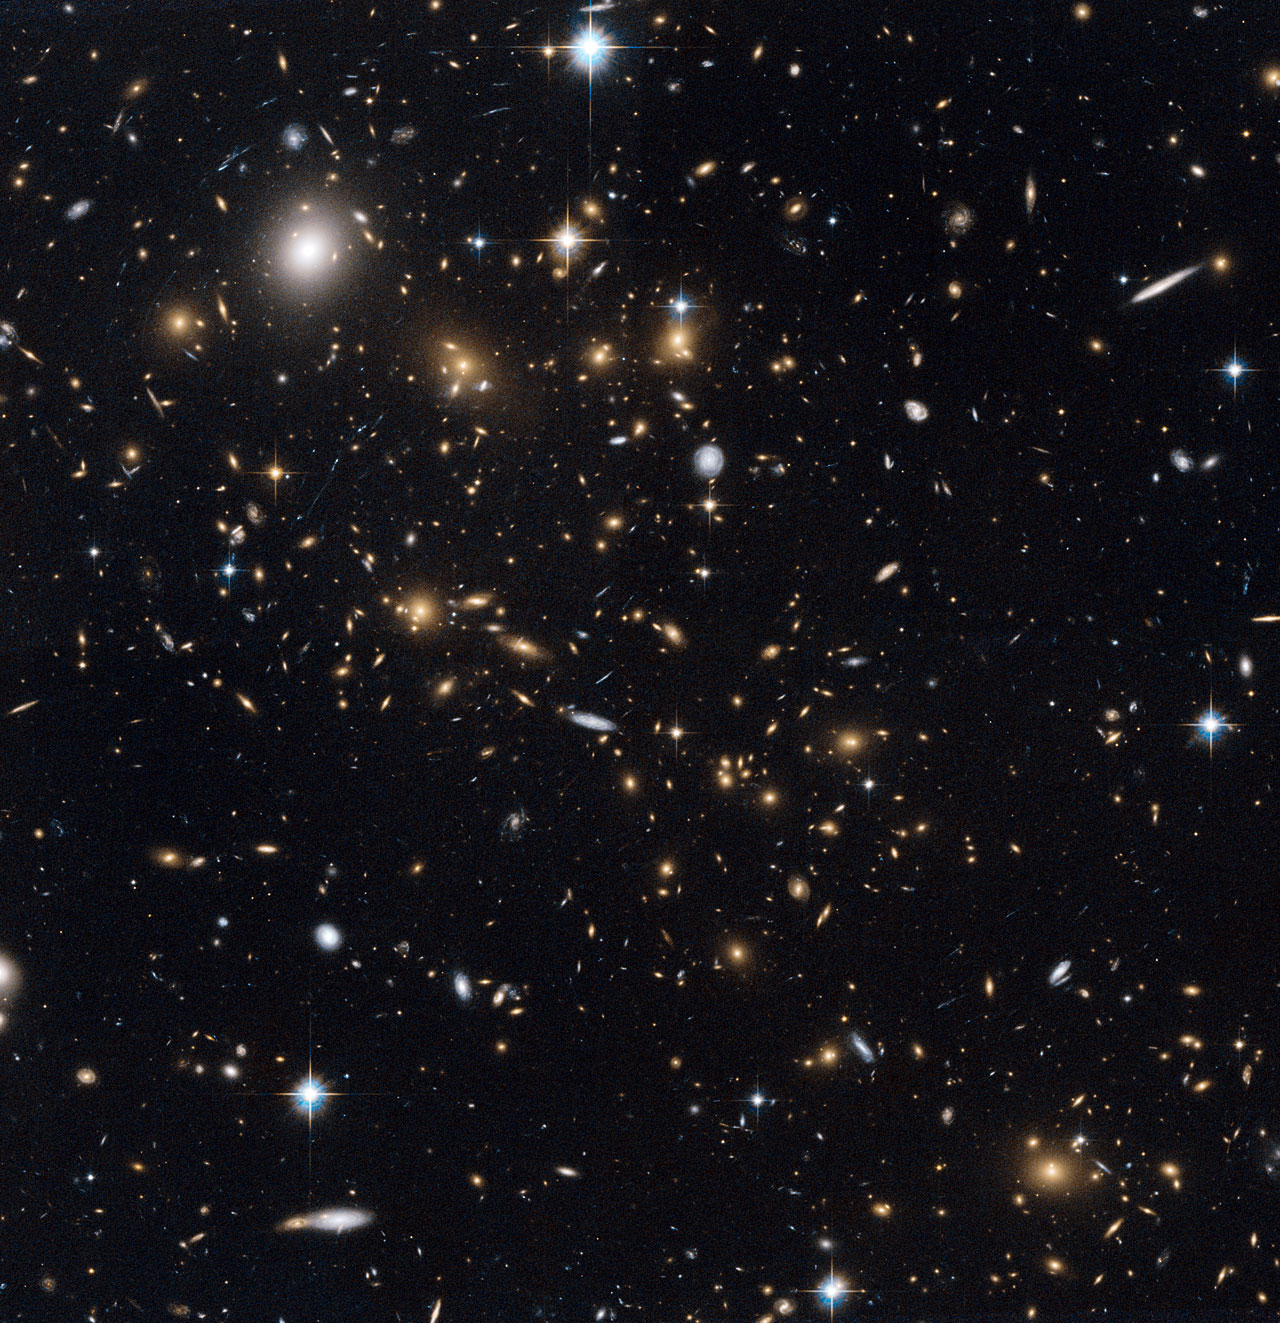
\includegraphics[width=\textwidth]{macs-cluster.jpg}
                \newline
                {\tiny NASA/ESA}
            \end{center}
        \end{column}
    \end{columns}
}


\frame
{
    \frametitle{Weak Lensing Limitations}

    \begin{columns}
        \begin{column}{0.5\textwidth}    
            \begin{itemize}

                \item It is a weak effect in general (other than special cases)

                \item Statistical approach is required: average signal from
                    many lenses and many backgroudn sources

                \item But these are unimportant limitations. The theory doesn't
                    predict anything about individual objects anyway: these are
                    messy systems with a complicated history

            \end{itemize}
        \end{column}
        \begin{column}{0.5\textwidth}
            \begin{center}
                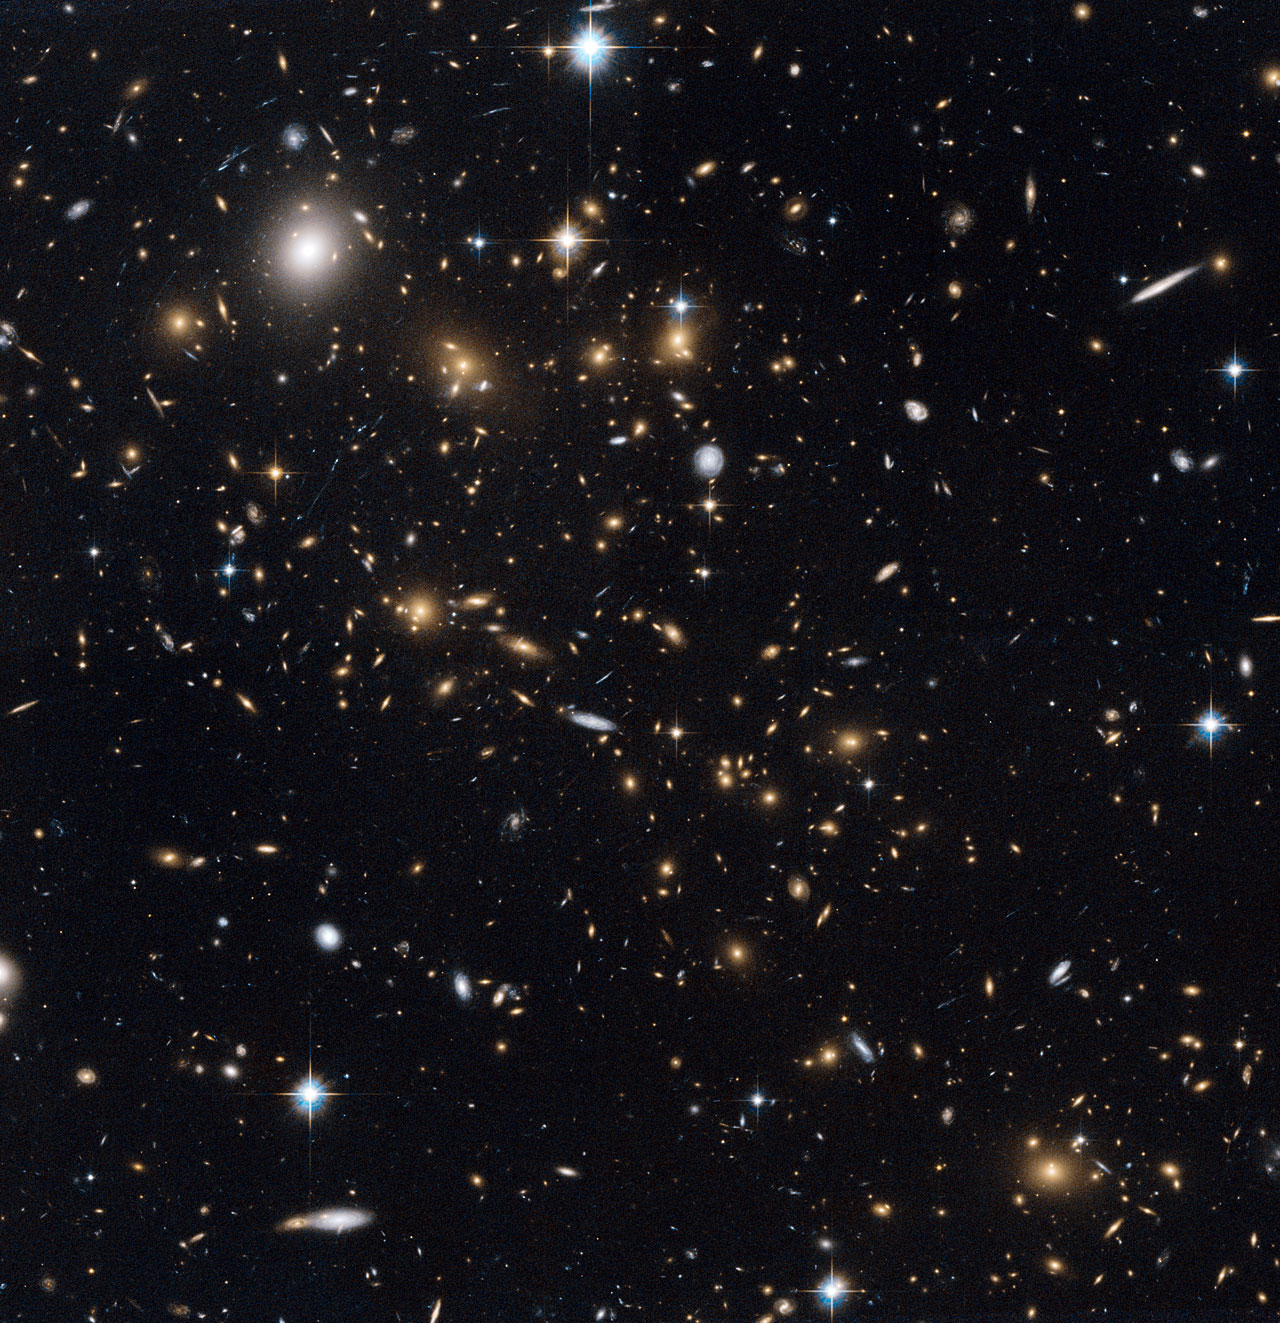
\includegraphics[width=\textwidth]{macs-cluster.jpg}
                \newline
                {\tiny NASA/ESA}
            \end{center}
        \end{column}
    \end{columns}
}





\end{document}
